%======================================================================
% Quantum Geometric Effects at the Monkey Saddle -- thesis talk
% 20 min talk + 5 min Q&A, 16:9, beamer. Plain-language version.
% Compile:  pdflatex main  (twice)
%======================================================================
\documentclass[aspectratio=169,11pt]{beamer}

\usepackage[T1]{fontenc}
\usepackage{lmodern}
\usepackage{amsmath,amssymb,bm}
\usepackage{graphicx}
\usepackage{booktabs}
\usepackage{tikz}
\usepackage{appendixnumberbeamer}

\graphicspath{{figures/}{logos/}}

%---------------------------------------------------------------------- look
\usetheme{default}
\usefonttheme{professionalfonts}
\definecolor{navy}{HTML}{1F3A68}
\definecolor{ochre}{HTML}{B8742A}
\definecolor{paper}{HTML}{FFFFFF}
\definecolor{ink}{HTML}{1A1A1A}
\definecolor{muted}{HTML}{5A5A5A}
\definecolor{boxbg}{HTML}{EEF2F8}

\setbeamercolor{normal text}{fg=ink,bg=paper}
\setbeamercolor{frametitle}{fg=navy}
\setbeamercolor{structure}{fg=navy}
\setbeamercolor{alerted text}{fg=ochre}
\setbeamercolor{caption name}{fg=navy}
\setbeamerfont{frametitle}{size=\large,series=\bfseries}
\setbeamerfont{caption}{size=\footnotesize}
\setbeamertemplate{navigation symbols}{}
\setbeamertemplate{itemize items}{\textcolor{navy}{\raisebox{0.15ex}{\scriptsize$\blacksquare$}}}
\setbeamertemplate{enumerate items}[default]
\setbeamertemplate{caption}{\raggedright\usebeamerfont{caption}\color{muted}\insertcaption\par}

% frame title with a thin rule under it
\setbeamertemplate{frametitle}{%
  \vskip6pt\usebeamerfont{frametitle}\usebeamercolor[fg]{frametitle}\insertframetitle\par
  \vskip2pt{\color{navy}\rule{\textwidth}{0.6pt}}\vskip-2pt}

% footer: author | short title | page
\setbeamertemplate{footline}{%
  \leavevmode\hbox to\paperwidth{\color{muted}\tiny
    \hspace{0.4cm}\insertshortauthor\hfill\insertshorttitle\hfill
    \insertframenumber\,/\,\inserttotalframenumber\hspace{0.4cm}}\vskip5pt}

% a box for the one sentence the audience should remember
\newcommand{\keybox}[1]{%
  \begin{center}\colorbox{boxbg}{\parbox{0.94\linewidth}{\vskip3pt\centering #1\vskip3pt}}\end{center}}

% figure that keeps its aspect ratio: \fig[width]{height}{file}
\newcommand{\fig}[3][\linewidth]{\includegraphics[width=#1,height=#2,keepaspectratio]{#3}}

% logo slot: uses logos/<name>.png|.jpg|.pdf if present, else a labelled placeholder
\newcommand{\logoslot}[2]{%
  \IfFileExists{logos/#1.png}{\includegraphics[height=1.35cm,keepaspectratio]{#1.png}}{%
  \IfFileExists{logos/#1.pdf}{\includegraphics[height=1.35cm,keepaspectratio]{#1.pdf}}{%
  \IfFileExists{logos/#1.jpg}{\includegraphics[height=1.35cm,keepaspectratio]{#1.jpg}}{%
  \fbox{\parbox[c][1.2cm][c]{1.6cm}{\centering\tiny #2\\ logo}}}}}}

\newcommand{\bk}{\mathbf{k}}
\newcommand{\bq}{\mathbf{q}}
\newcommand{\chie}{\chi_{e}}
\newcommand{\chig}{\chi_{\rm geom}}
\newcommand{\chim}{\chi_{\rm mass}}
\newcommand{\Evhs}{E_{\rm vhs}}
\newcommand{\meV}{\,\mathrm{meV}}
\newcommand{\nm}{\,\mathrm{nm}}

%---------------------------------------------------------------------- info
\title[Quantum geometry at the monkey saddle]{Quantum Geometric Effects at the Monkey Saddle Lifshitz Point in Biased Bernal Bilayer Graphene}
\author[Rajat Shuvra Saha, CMT Group, SPS]{Rajat Shuvra Saha}
\date{M.Sc.\ Thesis Defence \quad$\cdot$\quad 25th November 2026}

\begin{document}
%======================================================================
% 1. COVER
%======================================================================
{
\usebackgroundtemplate{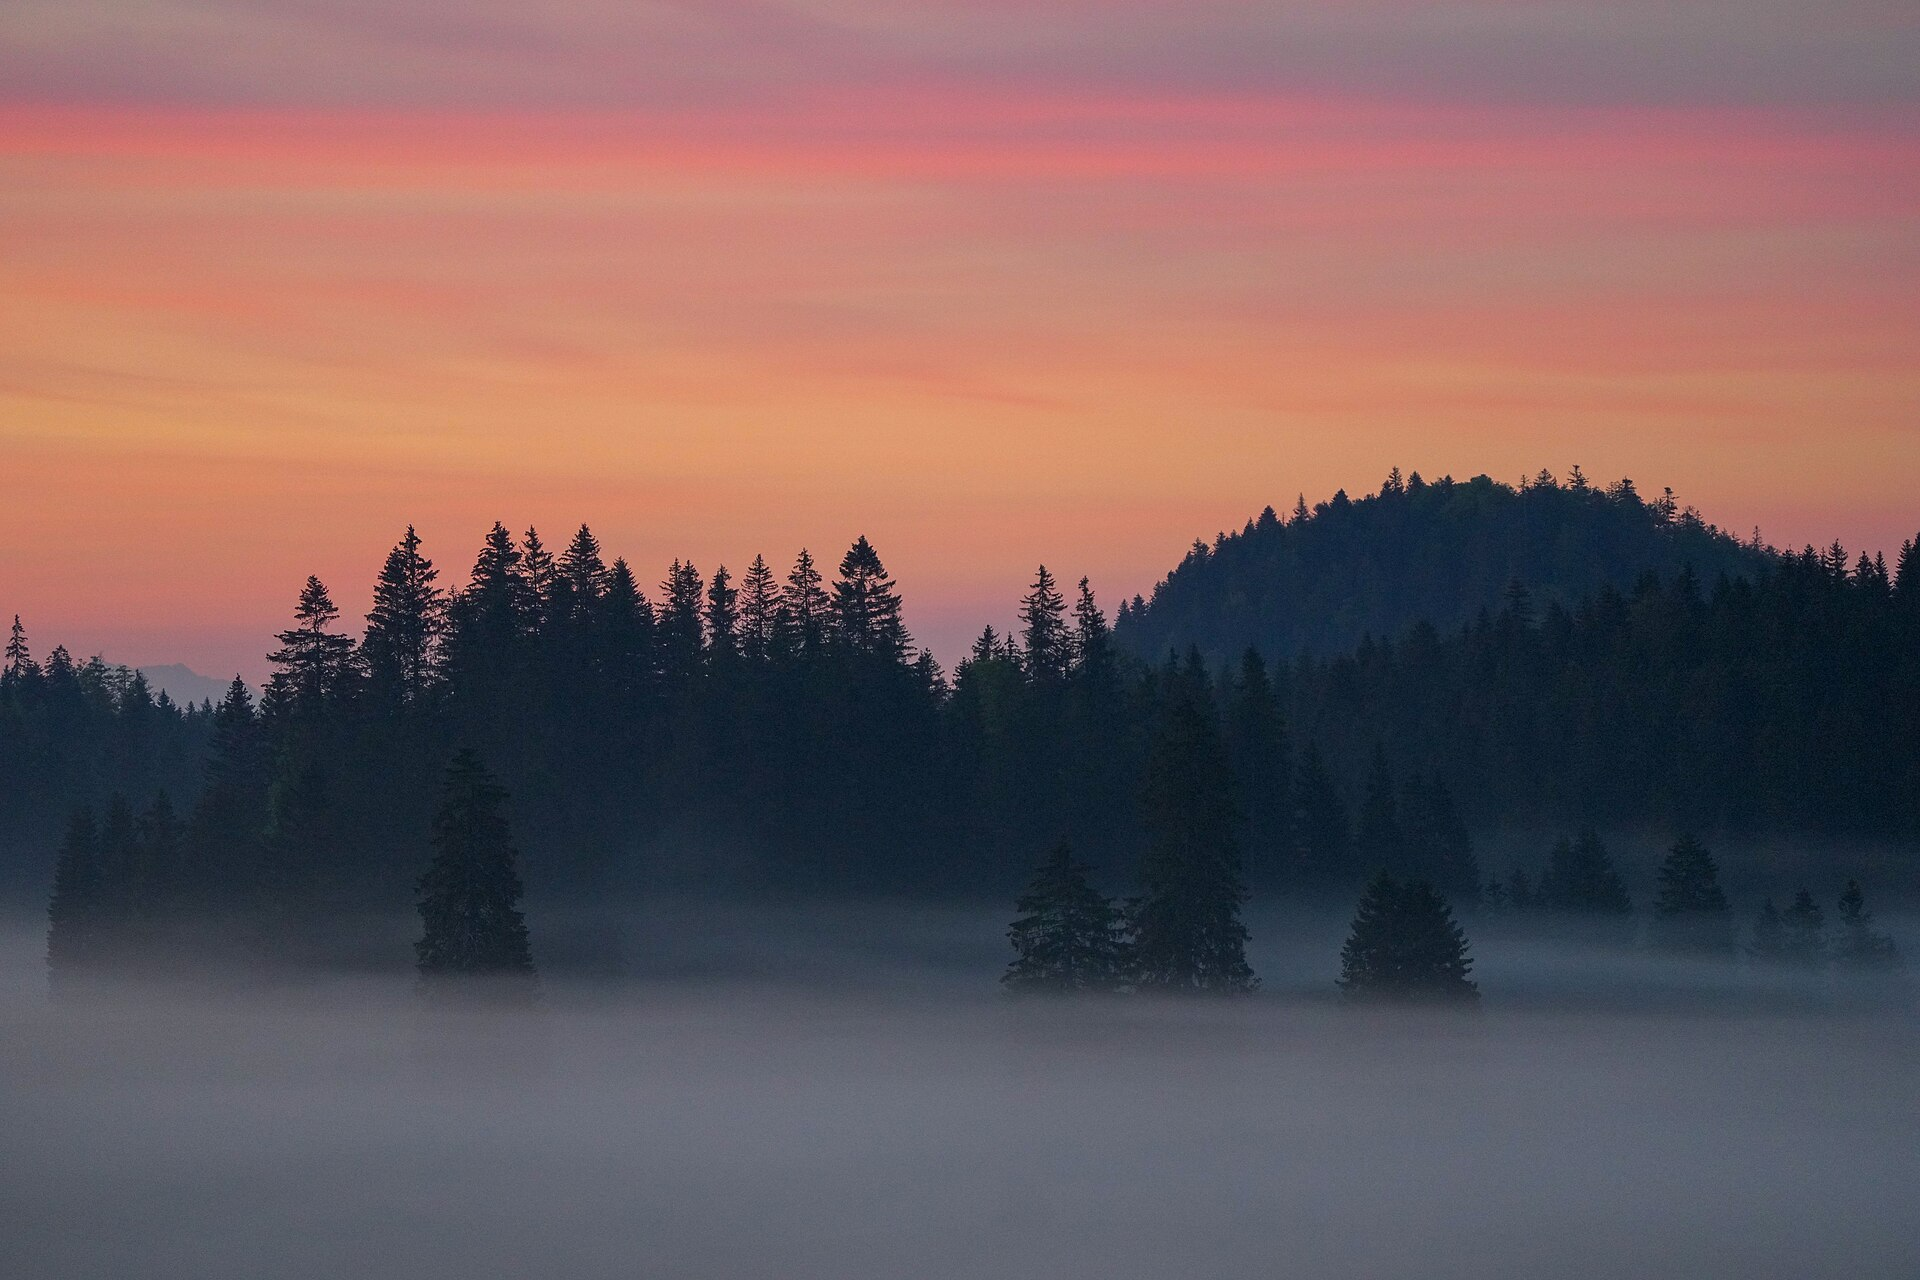
\includegraphics[width=\paperwidth,height=\paperheight]{cover_background.jpg}}
\setbeamertemplate{footline}{}
\begin{frame}[plain]
\centering
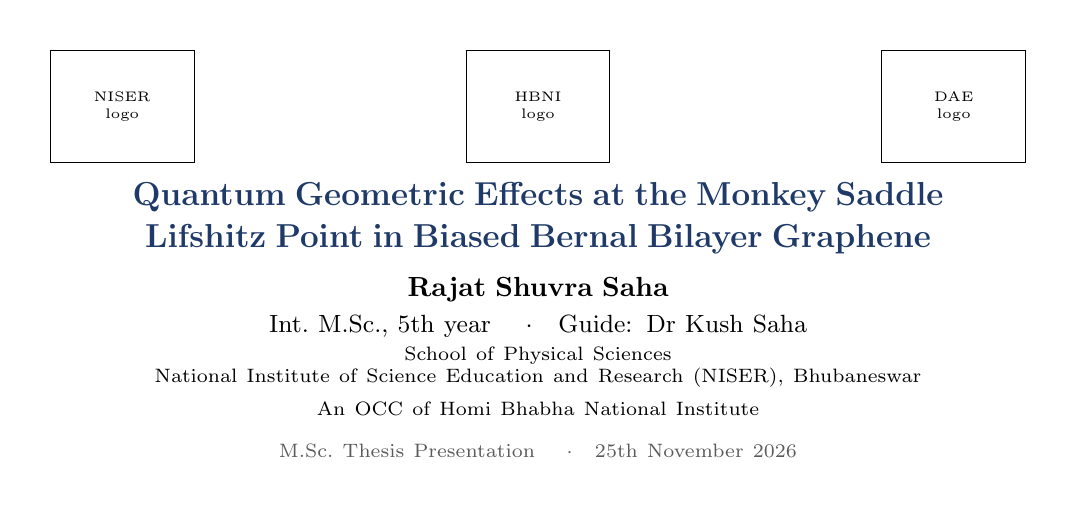
\begin{tikzpicture}
  \node[fill=white,fill opacity=0.88,text opacity=1,rounded corners=4pt,
        inner sep=8pt,text width=12.4cm,align=center] {%
    \logoslot{niser_logo}{NISER}\hfill
    \logoslot{hbni_logo}{HBNI}\hfill
    \logoslot{dae_logo}{DAE}\\[6pt]
    {\color{navy}\large\bfseries Quantum Geometric Effects at the Monkey Saddle\\[1pt]
     Lifshitz Point in Biased Bernal Bilayer Graphene\par}\vskip6pt
    {\normalsize\bfseries Rajat Shuvra Saha}\\[1pt]
    {\small Int.\ M.Sc., 5th year \quad$\cdot$\quad Guide: Dr Kush Saha}\\[2pt]
    {\scriptsize School of Physical Sciences\\
     National Institute of Science Education and Research (NISER), Bhubaneswar\\
     An OCC of Homi Bhabha National Institute}\\[3pt]
    {\scriptsize\color{muted} M.Sc.\ Thesis Presentation \quad$\cdot$\quad 25th November 2026}
  };
\end{tikzpicture}
\vskip1.6cm
\end{frame}
}

%======================================================================
\section{Background}
%======================================================================

% 2. What is known (1)
\begin{frame}{What is known (1): a band has an energy and a shape}
\begin{columns}[T]
\column{0.47\textwidth}\small
A Bloch state $H_0(\bk)|u_n(\bk)\rangle=\varepsilon_n(\bk)|u_n(\bk)\rangle$ carries two pieces of information.\\[6pt]
\textbf{The energy $\varepsilon_n(\bk)$.} It gives the velocity $\partial_\mu\varepsilon_n$ and the
effective mass $(\partial_\mu\partial_\nu\varepsilon_n)^{-1}$. Textbook quantities such as the Drude weight
$\tau n/m$ and the superfluid weight $D^s\approx n_s/m^*$ depend only on this.\\[6pt]
\textbf{The wavefunction $|u_n(\bk)\rangle$.} How it changes across $\bk$ is the band's geometry.
\column{0.49\textwidth}\small
The Berry curvature $\Omega_n$ gives the Hall conductance, $\sigma_{xy}=\tfrac{e^2}{h}N_{\rm Ch}$,
but it is only half of the story. The full object is the quantum geometric tensor
\[
Q_n^{\mu\nu}=\langle\partial_\mu u_n|1-P_n|\partial_\nu u_n\rangle=g_n^{\mu\nu}-\tfrac{i}{2}\Omega_n^{\mu\nu}.
\]
The real part, the \textbf{quantum metric}, measures how far apart two nearby states are:
\[
1-|\langle u_n(\bk)|u_n(\bk+d\bk)\rangle|^2\simeq g_n^{\mu\nu}\,dk_\mu dk_\nu .
\]
{\footnotesize It shows up in nonlinear optics and transport, multipole moments, Landau levels,
and, as below, in magnetism and superconductivity.}
\end{columns}
\end{frame}

% 3. What is known (2)
\begin{frame}{What is known (2): geometry in magnetism and superconductivity}
\begin{columns}[T]
\column{0.49\textwidth}\footnotesize
\textbf{Spin fluctuations.} In $\chi^0(\bq)$ every transition is weighted by $1-D_{nm}(\bk,\bq)$, the
quantum distance. The curvature at $q=0$ splits as $\chie=\chig+\chim$
{\color{muted}\tiny[Kitamura, Daido, Yanase 2024]}:
the Fermi-surface metric term $f'g$ always favours ferromagnetism, while the Fermi-sea
(positional-shift) term favours antiferromagnetism.\\[2pt]
In the Lieb lattice, near a band degeneracy, geometry alone turns an AFM-like
response into a ferromagnetic one. Graphene or Kane--Mele are not enough; the metric term needs a
large Fermi surface near a degeneracy. With RPA and Eliashberg theory this favours spin-triplet pairing.
\column{0.47\textwidth}\footnotesize
\textbf{Superfluid weight.} Without interband pairing, $D^s=D^{\rm conv}+D^{\rm geom}$
{\color{muted}\tiny[Peotta, T\"orm\"a 2015]}. The geometric part comes from interband terms and, for an
isolated band, is bounded below by $|N_{\rm Ch}|$: a flat band can still superconduct.\\[3pt]
\textbf{Monolayer FeSe on SrTiO$_3$.} $T_c$ rises from about $10$\,K (bulk) to $65$--$83$\,K, but zero resistance
appears near $40$\,K, because in 2D it is set by $T_{\rm BKT}=\pi D^s/8$.
With a sign-changing ($s_{\pm}$) gap and entangled bands (glide-mirror breaking in FeSe),
$D^{\rm geom}$ can turn \emph{negative}, pointing towards FFLO pairing.
\end{columns}
\vskip2pt
\keybox{\footnotesize\textbf{Open gap:} geometric ferromagnetism was shown at a \emph{band touching} ($g\to\infty$).
What happens at a higher-order saddle, where the band is gapped and $g$ is finite?}
\end{frame}

% 4. Question
\begin{frame}{Where this fits and the question}
\begin{columns}[T]
\column{0.56\textwidth}\small
\textbf{Higher-order van Hove points.}
When ordinary saddles merge, the density of states diverges as a power law
{\color{muted}\scriptsize[Shtyk, Goldstein, Chamon 2017; Yuan, Isobe, Fu 2019]}.\\[6pt]
\textbf{Bernal bilayer graphene.}
A gate pushes the conduction band through such a point. Experiments see a cascade of
isospin-polarised metals and spin-polarised superconductivity there
{\color{muted}\scriptsize[Zhou \emph{et al.}\ 2022; Seiler \emph{et al.}\ 2022; de la Barrera \emph{et al.}\ 2022]}.\\[6pt]
So this is a natural place to test the geometric mechanism in a real, gate-tunable material.
\column{0.40\textwidth}
\vskip10pt
\keybox{\small\textbf{Question}\\[4pt]
At the monkey saddle, does the quantum metric decide the sign of $\partial_q^2\chi^0|_{q=0}$?\\[4pt]
In short: are the ferromagnetic fluctuations here caused by \textbf{geometry}
or by the \textbf{shape of the band}?}
\end{columns}
\end{frame}

%======================================================================
\section{Model}
%======================================================================

% 5.
\begin{frame}{The gate tunes the band through a Lifshitz point}
\begin{columns}[c]
\column{0.60\textwidth}\small
Four-band model, valley $K$, basis $(A_1,B_1,A_2,B_2)$, $\pi=k_x+ik_y$:
{\footnotesize\[
H=\begin{pmatrix}
V/2 & v\pi^\dagger & 0 & v_3\pi\\
v\pi & V/2 & \gamma_1 & 0\\
0 & \gamma_1 & -V/2 & v\pi^\dagger\\
v_3\pi^\dagger & 0 & v\pi & -V/2
\end{pmatrix}
\]}
\vskip-4pt{\footnotesize $v=0.658$\,eV\,nm, $\gamma_1=0.40$\,eV, $v_3=0.1v$. $H$ is linear in $\bk$, so every band derivative is an exact sum over four states.}
\[
\varepsilon_3-\tfrac V2\simeq\alpha k^2-Ak^3\cos3\varphi+Bk^4,\quad
\alpha=\underbrace{\tfrac{v_3^2}{V}}_{A_1\to B_2}-\underbrace{\tfrac{v^2V}{\gamma_1^2}}_{\rm dimer}
\]
{\footnotesize The two terms in $\alpha$ cancel at $V_c=\gamma_1v_3/v=40\meV$. \ $k_*=A/B=0.122\nm^{-1}$, $E_*=6.40\meV$, $\delta\equiv V/V_c$.}
\column{0.36\textwidth}
\begin{figure}
\centering\fig{4.4cm}{Monkey_Saddle_3D_Plot.png}
\caption{$\varepsilon_3$ at $V_c$. The $k^2$ term is gone, leaving a cubic ``monkey'' saddle.}
\end{figure}
\end{columns}
\end{frame}

% 6.
\begin{frame}{Three saddle phases and an $|E|^{-1/3}$ density of states}
\begin{columns}[T]
\column{0.49\textwidth}\centering
\fig{2.55cm}{Undergapped_state.png}\\[-2pt]{\scriptsize (a) $\delta=0.5$: minimum at $\bk=0$, three saddles}\\[3pt]
\fig{2.55cm}{Overgapped.png}\\[-2pt]{\scriptsize (c) $\delta=1.5$: maximum at $\bk=0$, saddles rotated by $\pi/3$}
\column{0.49\textwidth}\centering
\fig{2.55cm}{{Delta=1.0}.png}\\[-2pt]{\scriptsize (b) $\delta=1$: the three saddles merge}\\[4pt]
\begin{minipage}{0.97\linewidth}\small
Saddle energy $\Evhs-V/2\simeq4\alpha^3/27A^2$, at $|\bk_s|=2|\alpha|/3A$.\\[2pt]
At $V_c$ I could do the integral exactly:
\keybox{\footnotesize
$\nu(E)=\dfrac{B(\frac12,\frac16)}{12\pi^2}\,A^{-2/3}|E-E_c|^{-1/3}$\\[3pt]
$\chi^0(0)\simeq0.0702\,A^{-2/3}T^{-1/3}$, within $1\%$ of the numerics}
\end{minipage}
\end{columns}
\end{frame}

%======================================================================
\section{Quantum geometry}
%======================================================================

% 7.
\begin{frame}{At the saddle the two channels add in $g$ and cancel in $\Omega$}
\small
At $\bk=0$ the band state is just $|A_1\rangle$, and only the two channels that appear in $\alpha(V)$ contribute:
\[
g_{xx}=g_{yy}=\frac{v_3^2}{V^2}\;{\color{navy}+}\;\frac{v^2(\gamma_1^2+V^2)}{\gamma_1^4},\qquad
\Omega_{xy}=\frac{2v_3^2}{V^2}\;{\color{ochre}-}\;\frac{2v^2(\gamma_1^2+V^2)}{\gamma_1^4}
\]
\begin{columns}[c]
\column{0.46\textwidth}
\begin{table}\scriptsize
\begin{tabular}{@{}ccccc@{}}
\toprule
$\delta$ & $\alpha$ & $g_{xx}$ & $\Omega_{xy}$ & dimer share\\
 & (eV\,nm$^2$) & (nm$^2$) & (nm$^2$) & of $g$\\
\midrule
0.5 & $+0.162$ & 13.54 & $+16.22$ & 0.20\\
1.0 & $0$ & 5.44 & $-0.05$ & 0.50\\
1.5 & $-0.090$ & 3.97 & $-3.13$ & 0.69\\
\bottomrule
\end{tabular}
\end{table}
\column{0.50\textwidth}\footnotesize
\begin{itemize}\setlength{\itemsep}{3pt}
\item $B_2$ couples through $\pi$ and the dimer through $\pi^\dagger$, so they have \textbf{opposite chirality}.
      Each one saturates $|\Omega|\le2\sqrt{\det g}$.
\item The same balance that kills the effective mass also kills $\Omega$ (up to $O(V^2/\gamma_1^2)$).
\item Away from $\bk=0$, $g$ and $\Omega$ sit in lobes near $|\bk|\approx k_*$.
\end{itemize}
So the critical band is \textbf{metric dominated}, and it is $g$, not $\Omega$, that enters the spin response.
\end{columns}
\end{frame}

%======================================================================
\section{GES}
%======================================================================

% 8.
\begin{frame}{Splitting the curvature of the spin susceptibility}
\small
Bare spin bubble (per spin, per valley), with $\bk_\pm=\bk\pm\bq/2$:
\[
\chi^0(\bq)=-\sum_{nm}\int\!\frac{d^2k}{(2\pi)^2}\,
\frac{f(\varepsilon_{n\bk_-})-f(\varepsilon_{m\bk_+})}{\varepsilon_{n\bk_-}-\varepsilon_{m\bk_+}}
\,\big|\langle u_{n\bk_-}|u_{m\bk_+}\rangle\big|^2
\]
\[
\chie\equiv\partial_{q_x}^2\chi^0\big|_{0}=\chig+\chim,\qquad
\chi^0(\bq)\simeq\chi^0(0)(1-\ell^2q^2),\quad \ell^2=-\chie/2\chi^0(0)
\]
\[
\chig=2\sum_n\int_{\bk}\Big[\frac{f'_n}{2}\,g^n_K+f_n\,X_n\Big],\qquad
\chim=-2\sum_n\int_{\bk}\frac{f''_n}{12}\,[m_n^{-1}]
\]
\begin{columns}[T]
\column{0.52\textwidth}\footnotesize
$g_K=2g_{\hat q\hat q}$;\;
$X_n=\sum_{m\neq n}\dfrac{2|v^{\hat q}_{nm}|^2}{(\varepsilon_m-\varepsilon_n)(\varepsilon_n-\varepsilon_m)^2}$;\;
$[m_n^{-1}]=\partial_{\hat q}^2\varepsilon_n$.
\column{0.44\textwidth}\footnotesize
In RPA, $\chi_s=\chi^0/(1-U\chi^0)$. If $\chie<0$, $q=0$ is a peak, and the Stoner instability happens there first.
\end{columns}
\end{frame}

% 9.
\begin{frame}{How to tell geometry from dispersion}
\begin{columns}[T]
\column{0.50\textwidth}\small
\textbf{Metric term.} $f'\le0$, so $\tfrac12f'g_K$ is always negative: geometry pushes towards $q=0$.
The Fermi-sea term $X_n$ partly undoes this.\\[8pt]
\textbf{Mass term.} $f''$ is odd about $\mu$, so $\chim$ compares the band curvature just below
and just above $\mu$. At a saddle the curvature is large and flips sign, so $\chim$ is large and flips sign at $\Evhs$.
\column{0.46\textwidth}
\vskip6pt
\keybox{We call the fluctuation \textbf{geometry driven} when
\[\chie<0<\chim\]
\small The band shape alone would give a dip at $q=0$; the wavefunction overlaps turn it into a peak.}
\vskip4pt
{\scriptsize\color{muted}Numerics: $60^\circ$ wedge, Gauss--Legendre polar grids, full Fermi functions on all four bands, Fermi-sea tail extrapolated in $1/k_{\max}$ (backup).}
\end{columns}
\end{frame}

%======================================================================
\section{Results}
%======================================================================

% 10.
\begin{frame}{Near the saddle the band shape wins; at higher density, geometry does}
\begin{columns}[c]
\column{0.62\textwidth}
\centering\fig{6.5cm}{GES_ipynb_Biased.png}
\column{0.36\textwidth}
\footnotesize
\textbf{Top, near $\Evhs$:} both terms are about $10$\,eV$^{-1}$, but $\chim$ flips sign at $\Evhs$ and
decides the sign of $\chie$. The FM window is mostly dispersion driven (grey), with a thin geometric strip (orange).\\[6pt]
\textbf{Bottom, higher density:} $\chim>0$, yet $|\chig|>\chim$ once $\mu-V/2\gtrsim4.2\meV$, for every $\delta$.\\[6pt]
Example, $8\meV$ at $V_c$: $\chie=-0.30$, $\chim=+1.57$\,eV$^{-1}$, so switching geometry on takes $\ell^2$ from $-6.8$ to $+1.3\nm^2$.\\[6pt]
{\color{muted}\scriptsize $T=0.1\meV$; $\delta=0.8,1,1.2$.}
\end{columns}
\end{frame}

% 11.
\begin{frame}{At $\Evhs$, geometry decides only above $V_c$ and at low $T$}
\begin{figure}
\centering
\begin{minipage}[t]{0.32\linewidth}\centering\fig{3.4cm}{chi_geom_Temperature_Scan_Biased.png}\\{\scriptsize (a) $\chig$}\end{minipage}\hfill
\begin{minipage}[t]{0.32\linewidth}\centering\fig{3.4cm}{chi_mass_Temperature_Scan_Biased.png}\\{\scriptsize (b) $\chim$}\end{minipage}\hfill
\begin{minipage}[t]{0.32\linewidth}\centering\fig{3.4cm}{chi_total_temp_scan_biased.png}\\{\scriptsize (c) $\chie$}\end{minipage}
\end{figure}
\vskip-6pt
\footnotesize
\begin{columns}[T]
\column{0.32\textwidth} \textbf{$\delta=0.5$:} $\chim\to-65$, $\chie\to-83$\,eV$^{-1}$. Strong, but from the \emph{band shape}.
\column{0.32\textwidth} \textbf{$\delta=1$:} $\chie>0$ below $1.8$\,K ($\chim=+26$ against $\chig=-14$). Geometry wins only between $1.9$ and $2.5$\,K.
\column{0.32\textwidth} \textbf{$\delta=1.5$:} $\chie<0$ at all $T$, and $\chim>0$ below $5$\,K, so here it is \emph{geometry}.
\end{columns}
\vskip4pt
{\scriptsize\color{muted}$\mu=\Evhs$, $1.16$--$116$\,K. $\chig$ changes sign at 16, 34 and 63\,K, when thermally occupied valence states let the Fermi-sea term win.}
\end{frame}

% 12.
\begin{frame}{A direct check: the split is right, but $q=0$ is only a local peak}
\begin{figure}
\centering\fig[0.92\linewidth]{3.3cm}{fullfour_band_comparison_ipynb.png}
\caption{$\chi^0(q\hat x)$ at $V_c$, $\mu-V/2=8\meV$, $T=0.2\meV$. Solid: four-band model. Dashed: same energies, but overlaps set to $\delta_{nm}$.}
\end{figure}
\vskip-6pt
\begin{columns}[T]
\column{0.48\textwidth}\scriptsize
\begin{tabular}{@{}lcc@{}}
\toprule
curvature at $q\to0$ & bubble & formula\\
\midrule
full model & $-0.152$ & $\chie/2=-0.151$\\
trivial overlaps & $+0.790$ & $\chim/2=+0.788$\\
\bottomrule
\end{tabular}
\column{0.50\textwidth}\footnotesize
\begin{itemize}\setlength{\itemsep}{2pt}
\item This check does not use the GES formulas at all.
\item The true maximum is at $q\approx0.28\nm^{-1}$, about $15\%$ above $\chi^0(0)$. In RPA a finite-$q$ instability would come first.
\end{itemize}
\end{columns}
\end{frame}

% 13.
\begin{frame}{Map of the $q=0$ response at $V_c$}
\begin{figure}
\centering\fig[0.9\linewidth]{3.6cm}{Monkey_Saddle_Phase_Diagram.png}
\caption{Orange: geometry driven ($\chie<0<\chim$). Brown: band-shape driven ($\chie<0$, $\chim<0$). Cream: $q=0$ is a minimum of $\chi^0$.}
\end{figure}
\vskip-4pt
\small
\begin{itemize}\setlength{\itemsep}{2pt}
\item Near the saddle, geometry wins only in a thin strip, which moves to higher $\mu$ as $T$ rises.
\item At higher density there is a large geometric region starting at $\mu-V/2\approx4.2\meV$, almost independent of $T$ up to $0.7\meV$.
\end{itemize}
\end{frame}

%======================================================================
\section{Discussion}
%======================================================================

% 14.
\begin{frame}{Singular in energy, regular in geometry}
\begin{columns}[c]
\column{0.52\textwidth}\small
\textbf{Band-touching saddle} (Kitamura model, which I reproduced): $g\propto1/p^2$, and as the gap
$\Delta\to0$, $\chig$ grows past a positive $\chim$.\\[6pt]
\textbf{Monkey saddle:} the dispersion is singular, but the band is gapped by $V$ and
$g=5.44\nm^2$ stays finite. Near $\Evhs$, $\chim$ is large and flips sign, so geometry can only tip the
balance where the band shape is close to neutral.\\[6pt]
\keybox{\small A higher-order saddle boosts the density of states. To get geometry-driven magnetism you
also need a \textbf{small gap to another band at the saddle}.}
\column{0.44\textwidth}
\begin{figure}
\centering\fig{4.5cm}{GES_Singular.png}
\caption{Gapped band-touching saddle at $\mu=E_s$: $\chig$, $\chim$, $\chie$ against $T$ for $\Delta=0.17$ and $0.02$.}
\end{figure}
\end{columns}
\end{frame}

% 15.
\begin{frame}{Limitations and next steps}
\begin{columns}[T]
\column{0.50\textwidth}\small
\textbf{What I have not done}
\begin{itemize}\setlength{\itemsep}{3pt}
\item Bare bubble only, interactions only through RPA. Vertex corrections could change which of $q=0$ and $q\approx0.28\nm^{-1}$ wins.
\item One valley and one spin. Intervalley (isospin) channels, which matter for the observed cascades, are left out.
\item Minimal hoppings ($v,\gamma_1,v_3$). Adding $\gamma_4$ and $\Delta'$ moves $V_c$; I expect, but have not shown, that the chirality argument survives.
\end{itemize}
\column{0.46\textwidth}\small
\textbf{Next steps}
\begin{itemize}\setlength{\itemsep}{3pt}
\item Full $\mathrm{SU}(4)$ isospin susceptibility with both valleys.
\item Follow the finite-$q$ peak into an ordered state, beyond RPA.
\item Compare the $(\mu,V)$ windows with measured gate-tuned phase diagrams.
\end{itemize}
\end{columns}
\end{frame}

% 16. Key results
\begin{frame}{Key results}
\begin{enumerate}\small\setlength{\itemsep}{2pt}
\item \textbf{Exact density of states.} At $V_c=40\meV$ the saddle is cubic and
      $\nu(E)=\frac{B(1/2,1/6)}{12\pi^2}A^{-2/3}|E-E_c|^{-1/3}$. It gives $\chi^0(0)\propto T^{-1/3}$, within $1\%$ of the numerics.
\item \textbf{Closed-form geometry.} The two channels that cancel in the effective mass \emph{add} in $g$ and
      \emph{cancel} in $\Omega$: $g=5.44\nm^2$, and $\Omega_{xy}=0$ at $V=0.995\,V_c$.
\item \textbf{The split is checked.} $\chie=\chig+\chim$ agrees with a direct finite-$q$ bubble to better than $1\%$.
\item \textbf{Geometry decides only part of the map.} Near $\Evhs$ the band shape sets the sign. Geometry wins for
      $\mu-V/2\gtrsim4.2\meV$ at every bias, and at $\Evhs$ only for $V>V_c$ and $T\lesssim5$\,K.
\item \textbf{Caveat.} Where geometry wins, $q=0$ is a local peak only; the largest response is at $q\approx0.28\nm^{-1}$.
\end{enumerate}
\keybox{\footnotesize The monkey saddle realises the Kitamura--Daido--Yanase mechanism in a gapped, gate-tunable band,
but as a \textbf{correction} to a response that is mostly set by the band shape.}
\end{frame}

% 17. Thanks
{
\usebackgroundtemplate{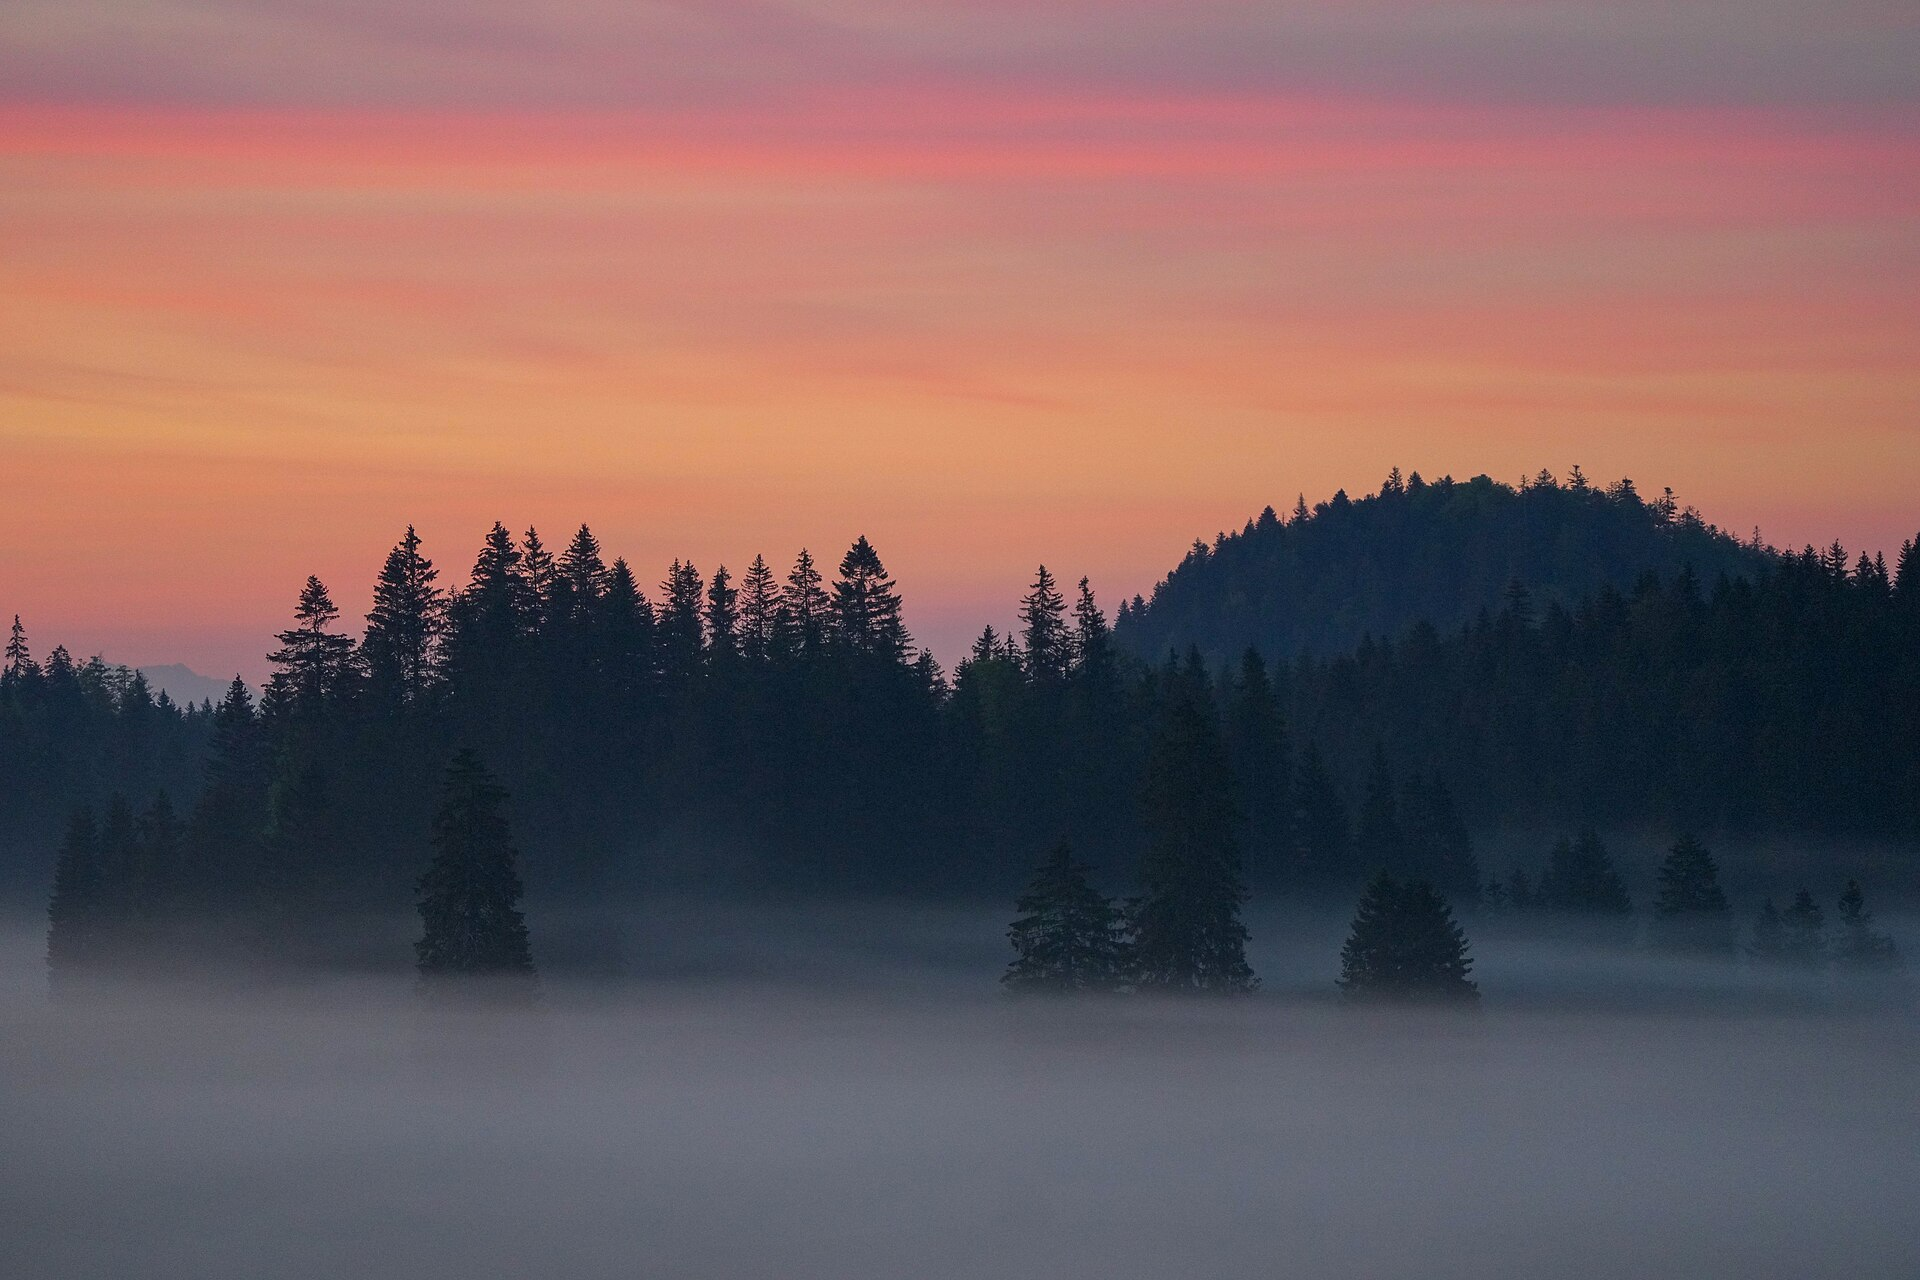
\includegraphics[width=\paperwidth,height=\paperheight]{cover_background.jpg}}
\setbeamertemplate{footline}{}
\begin{frame}[plain]
\begin{tikzpicture}[remember picture,overlay]
  \node[fill=white,fill opacity=0.88,text opacity=1,rounded corners=4pt,inner sep=12pt,align=center]
        at ([yshift=-3.0cm]current page.north) {%
    {\color{navy}\LARGE\bfseries Thank you}\\[6pt]
    {\normalsize Questions?}\\[8pt]
    {\footnotesize I thank Dr Kush Saha, Reader-F, and Akash Dey, RA (SPS), for their help with this project.}};
\end{tikzpicture}
\end{frame}
}

\appendix
\section{Backup}
%======================================================================

\begin{frame}{Backup: conventions and consistency checks}
\small
\begin{itemize}\setlength{\itemsep}{5pt}
\item All susceptibilities per spin and per valley; $K'$ identical by time reversal.
\item $g_K\equiv2g_{\hat q\hat q}$, with $g$ the standard metric of the QGT. $C_3$: every tensor evaluated as $(xx+yy)/2$.
\item $X_n$ and the $\tfrac1{12}f''$ coefficient obtained by expanding the bubble to $O(q^2)$ (Backup C).
\item The normalisation of every term is fixed independently by the finite-$q$ check:
      $-0.152$ vs.\ $-0.151$ (full) and $+0.790$ vs.\ $+0.788$ (trivial overlaps).
\item $\chi^0(0)$ vs.\ analytic $T^{-1/3}$ law: $1.111/1.109$, $0.815/0.817$, $0.642/0.649$ at $T=0.02,0.05,0.1\meV$.
\item Convergence: inner cutoff $0.6\to0.8\nm^{-1}$ and $+1/3$ angular points change no quoted digit.
\end{itemize}
\end{frame}


\begin{frame}{Backup: references}
\scriptsize
\begin{itemize}\setlength{\itemsep}{3pt}
\item L. Van Hove, Phys.\ Rev.\ \textbf{89}, 1189 (1953).
\item E.\,C. Stoner, Proc.\ R.\ Soc.\ Lond.\ A \textbf{165}, 372 (1938).
\item N.\,F.\,Q. Yuan, H. Isobe and L. Fu, Nat.\ Commun.\ \textbf{10}, 5769 (2019).
\item A. Shtyk, G. Goldstein and C. Chamon, Phys.\ Rev.\ B \textbf{95}, 035137 (2017).
\item H. Zhou \emph{et al.}, Science \textbf{375}, 774 (2022).
\item A.\,M. Seiler \emph{et al.}, Nature \textbf{608}, 298 (2022).
\item S.\,C. de la Barrera \emph{et al.}, Nat.\ Phys.\ \textbf{18}, 771 (2022).
\item T. Kitamura, A. Daido and Y. Yanase, Phys.\ Rev.\ Lett.\ (2024); arXiv:2304.11536.
\item S. Peotta and P. T\"orm\"a, Nat.\ Commun.\ \textbf{6}, 8944 (2015).
\item P. T\"orm\"a, S. Peotta and B.\,A. Bernevig, Nat.\ Rev.\ Phys.\ \textbf{4}, 528 (2022).
\item E. McCann and V.\,I. Fal'ko, Phys.\ Rev.\ Lett.\ \textbf{96}, 086805 (2006).
\item E. McCann and M. Koshino, Rep.\ Prog.\ Phys.\ \textbf{76}, 056503 (2013).
\item J.\,P. Provost and G. Vallee, Commun.\ Math.\ Phys.\ \textbf{76}, 289 (1980).
\end{itemize}
\end{frame}

% --- Appendix A
\begin{frame}{Backup A1: effective two-band model}
For $|E|,\,vk\ll\gamma_1$, eliminate $(B_1,A_2)$:
\[
h(\bk)=\begin{pmatrix}\frac V2\big(1-\frac{2v^2k^2}{\gamma_1^2}\big) & X^*\\[2pt] X & -\frac V2\big(1-\frac{2v^2k^2}{\gamma_1^2}\big)\end{pmatrix},\qquad
X=v_3\pi-\frac{v^2}{\gamma_1}(\pi^\dagger)^2
\]
\[
|X|^2=v_3^2k^2-\frac{2v_3v^2}{\gamma_1}k^3\cos3\varphi+\frac{v^4}{\gamma_1^2}k^4
\]
Expanding $\varepsilon_3=\sqrt{(V/2)^2(1-2v^2k^2/\gamma_1^2)^2+|X|^2}$ for $|X|\ll V$:
\[
\varepsilon_3-\tfrac V2\simeq\Big(\tfrac{v_3^2}{V}-\tfrac{v^2V}{\gamma_1^2}\Big)k^2-\tfrac{2v_3v^2}{\gamma_1V}k^3\cos3\varphi+\tfrac{v^4}{\gamma_1^2V}k^4,
\qquad A=\frac{2v^3}{\gamma_1^2},\quad B=\frac{v^5}{\gamma_1^3v_3}
\]
\small Saddles at $k_s=2|\alpha|/3A$, $\;\Evhs-V/2=4\alpha^3/27A^2$; Hessian at $\bk=0$ is $2\alpha\,\mathbb 1$.
Exact diagonalisation reproduces $\alpha(V)$ to four digits.
\end{frame}

\begin{frame}{Backup A2: density of states at the monkey saddle}
At $V_c$, $\varepsilon(\bk)=-Ak^3\cos3\varphi$. Root at $k_E=(|E|/A|\cos3\varphi|)^{1/3}$, with $|\partial_k\varepsilon|=3|E|/k_E$:
\[
\nu(E)=\frac{1}{4\pi^2}\int_0^{2\pi}\!d\varphi\,\frac{k_E^2}{3|E|}\,\Theta(-E\cos3\varphi)
=\frac{J}{12\pi^2A^{2/3}}\,|E|^{-1/3}
\]
\[
J=2\int_0^{\pi/2}\cos^{-2/3}u\,du=B\!\left(\tfrac12,\tfrac16\right)\simeq7.286
\]
\[\boxed{\nu(E)\simeq0.0615\,A^{-2/3}|E-E_c|^{-1/3}}\]
\begin{itemize}\small\setlength{\itemsep}{3pt}
\item Symmetric and integrable; nodal-line divergence cut off by $Bk^4$ at relative order $(|E|/E_*)^{1/3}$.
\item Four-band histogram agrees to $4\%$ at $0.2\meV$ and $12\%$ at $1\meV$.
\end{itemize}
\end{frame}

\begin{frame}{Backup A3: uniform susceptibility, $T^{-1/3}$ law}
\begin{columns}[c]
\column{0.44\textwidth}
\small
\[\chi^0(0)=\int dE\,\nu(E)\,[-f'(E-\mu)]\]
\[I=\int dx\,\frac{|x|^{-1/3}e^x}{(1+e^x)^2}\simeq1.142\]
\[\chi^0(0)\simeq0.0702\,A^{-2/3}T^{-1/3}\]
\footnotesize
\begin{tabular}{ccc}
\toprule
$T$ (meV) & analytic & numerics\\
\midrule
0.02 & 1.109 & 1.111\\
0.05 & 0.817 & 0.815\\
0.10 & 0.649 & 0.642\\
\bottomrule
\end{tabular}
\column{0.54\textwidth}
\begin{figure}
\centering\fig{3.6cm}{uniform_susceptibility_ipynb.png}
\caption{(a) $\chi^0(0)$ at $\Evhs$; dotted: $\propto T^{-1/3}$. (b) GES at $\mu-V/2=8\meV$. Solid: $\chie$; dashed: $\chim$.}
\end{figure}
\end{columns}
\end{frame}

% --- Appendix B
\begin{frame}{Backup B: quantum geometry at $\bk=0$}
Band 3 at $\bk=0$ is $|A_1\rangle$; velocities connect it only to $|B_2\rangle$ and $|B_1\rangle$:
\[
\langle A_1|\partial_xH|B_2\rangle=v_3,\ \ \langle A_1|\partial_yH|B_2\rangle=iv_3,\qquad
\langle A_1|\partial_xH|B_1\rangle=v,\ \ \langle A_1|\partial_yH|B_1\rangle=-iv
\]
\begin{itemize}\small\setlength{\itemsep}{4pt}
\item $B_2$ channel: $v_3^2/V^2$.
\item Dimer channel: $-v^2\,\partial_EG_{B_1B_1}\big|_{V/2}=v^2(\gamma_1^2+V^2)/\gamma_1^4$, with
      $G_{B_1B_1}(E)=\dfrac{E+V/2}{(E-V/2)(E+V/2)-\gamma_1^2}$.
\item $\mathrm{Im}[v^xv^y]=-v_3^2$ for $B_2$, $+v^2$ for $B_1$: opposite signs in $\Omega$.
\item Each channel saturates $|\Omega|\le2\sqrt{\det g}$; $\Omega_{xy}=0$ at $V\simeq0.995\,V_c$.
\end{itemize}
\end{frame}

% --- Appendix C
\begin{frame}{Backup C: derivation of the GES}
\footnotesize
\textbf{Energy factor.} With $a=\varepsilon(\bk_-)$, $b=\varepsilon(\bk_+)$:
\[
\frac{f(a)-f(b)}{a-b}=f'+\frac{q^2}{8}f''\partial^2\varepsilon+\frac{q^2}{24}f^{(3)}(\partial\varepsilon)^2+O(q^4)
\]
Integrating the last term by parts gives $-\tfrac1{12}f''\partial^2\varepsilon$ in the $q^2$ coefficient, hence $\chim$.
For linear $H$: $\;\partial_\mu\partial_\nu\varepsilon_n=\sum_{m\ne n}2\,\mathrm{Re}\,v^\mu_{nm}v^\nu_{mn}/(\varepsilon_n-\varepsilon_m)$ exactly.\\[6pt]
\textbf{Overlaps.} $m=n$: $\;1-q^2g^n_{\hat q\hat q}$ $\Rightarrow$ Fermi-surface term $f'g_K$.\\
$m\neq n$: $\;q^2|v^{\hat q}_{nm}|^2/(\varepsilon_n-\varepsilon_m)^2$ $\Rightarrow$ Fermi-sea term
\[
X_n=\sum_{m\neq n}\frac{2\,|v^{\hat q}_{nm}|^2}{(\varepsilon_m-\varepsilon_n)(\varepsilon_n-\varepsilon_m)^2}.
\]
By $C_3$ symmetry each quantity is evaluated as $(xx+yy)/2$.
\end{frame}

% --- Appendix D
\begin{frame}{Backup D: numerics and critical points}
\begin{columns}[T]
\column{0.38\textwidth}
\footnotesize
\begin{itemize}\setlength{\itemsep}{4pt}
\item Critical points on mirror lines; Brent root finding; exact Hessian.
\item Morse count (min $-$ saddle $+$ max) $=1$ in every phase.
\item $60^\circ$ wedge $\times6$; 12 Gauss--Legendre panels (64 nodes) on $k\le0.36\nm^{-1}$, 4 more to $0.6\nm^{-1}$; 48 angles.
\item Fermi-sea tail to $k_{\max}=20,80\nm^{-1}$, extrapolated in $1/k_{\max}$.
\item Larger cutoff / angular grid: no quoted digit changes.
\end{itemize}
\column{0.58\textwidth}
\scriptsize
\begin{tabular}{ccccc}
\toprule
$\delta$ & position & $|\bk|/k_*$ & $E-V/2$ (meV) & type\\
\midrule
0.5 & $\bk=0$ & 0 & 0 & minimum\\
0.5 & $\varphi=0$ & 0.158 & $+0.0174$ & saddle ($\times3$)\\
0.5 & $\varphi=0$ & 0.590 & $-0.239$ & minivalley ($\times3$)\\
1.0 & $\bk=0$ & 0 & 0 & monkey saddle\\
1.0 & $\varphi=0$ & 0.745 & $-0.657$ & minivalley ($\times3$)\\
1.5 & $\bk=0$ & 0 & 0 & maximum\\
1.5 & $\varphi=\pi$ & 0.170 & $-0.0140$ & saddle ($\times3$)\\
1.5 & $\varphi=0$ & 0.909 & $-1.336$ & minivalley ($\times3$)\\
\bottomrule
\end{tabular}
\end{columns}
\end{frame}

% --- Appendix E/F
\begin{frame}{Backup E: benchmark, the gapped singular saddle}
\begin{columns}[c]
\column{0.50\textwidth}
\small
\[
H(\mathbf p)=\tfrac{p^2}{2M}\sigma_0+\tfrac{p_xp_y}{M_{xy}}\sigma_x+\Delta\sigma_y+\tfrac{p_x^2-p_y^2}{2M_{xx}}\sigma_z
\]
\footnotesize $1/M=1$, $1/M_{xx}=0.5$, $1/M_{xy}=1.5$, cutoff $|\mathbf p|\le1$.
\begin{itemize}\footnotesize\setlength{\itemsep}{3pt}
\item $\Delta=0$: singular saddle at a band touching, $g\propto1/p^2$.
\item $\Delta\neq0$: gap $2\Delta$, four saddles at $E_s=-\Delta\sqrt{1-M_{xy}^2/M^2}$.
\item At $\mu=E_s$: $\chim>0$, $\chig<0$ and growing as $\Delta\to0$.
\item $\Delta=0.02$: $\chie<0$ at all $T$, geometry driven.
\end{itemize}
\column{0.46\textwidth}
\begin{figure}
\centering\fig{4.4cm}{Gapped_Singular_Saddle.png}
\caption{Bands of the benchmark model for $\Delta=0.17$ (model units).}
\end{figure}
\end{columns}
\end{frame}

\end{document}